\documentclass[a4paper,12pt]{report} %размер бумаги устанавливаем А4,     
\usepackage[14pt]{extsizes} %шрифт 14пунктов
\usepackage[T2A]{fontenc}
\usepackage[utf8]{inputenc} %включаем свою кодировку: koi8-r или utf8 в UNIX, cp1251 в Windows
\usepackage[english,russian]{babel} %используем русский и английский языки с переносами
\usepackage{amssymb,amsfonts,amsmath,mathtext,cite,enumerate,float} %подключаем нужные пакеты расширений
\usepackage[dvips]{graphicx} %хотим вставлять в диплом рисунки?
\usepackage{indentfirst} % абзац с отступом

\usepackage[labelfont=bf,justification=centering]{caption} % для
                                % классных подписей к графикам
\usepackage{subcaption}
\DeclareCaptionLabelFormat{gostfigure}{Рисунок #2}
\captionsetup[figure]{labelformat=gostfigure}
\DeclareCaptionLabelSeparator{gost}{.~}
\captionsetup{labelsep=gost}

\graphicspath{{images/}} %путь к рисункам
\makeatletter
\renewcommand{\@biblabel}[1]{#1.} % Заменяем библиографию с квадратных скобок на точку:
\makeatother
\newcommand{\tocsecindent}{\hspace{7mm}} % для введения выравнивание

\usepackage{geometry} % Меняем поля страницы
\geometry{left=2cm} % левое поле
\geometry{right=1.5cm} % правое поле
\geometry{top=1cm} % верхнее поле
\geometry{bottom=2cm} % нижнее поле

\makeatletter % Для вставки римских цифр в текст
\newcommand{\rmnum}[1]{\romannumeral #1}
\newcommand{\Rmnum}[1]{\expandafter\@slowromancap\romannumeral #1@}
\makeatother

\usepackage[usenames,dvipsnames]{color}
\usepackage[numbered,framed]{mcode} % Matlab код

\newcommand{\mychapter}[1]{\refstepcounter{chapter}
  \chapter*{\arabic{chapter} #1} \addcontentsline{toc}{chapter}{\arabic{chapter} #1}}  % убираем слова Глава

\linespread{1.3}  % 1.5 интервал

\renewcommand{\theenumi}{\arabic{enumi}} % Меняем везде перечисления на цифра.цифра
\renewcommand{\labelenumi}{\arabic{enumi}} % Меняем везде перечисления на цифра.цифра
\renewcommand{\theenumii}{.\arabic{enumii}} % Меняем везде перечисления на цифра.цифра
\renewcommand{\labelenumii}{\arabic{enumi}.\arabic{enumii}.} % Меняем везде перечисления на цифра.цифра
\renewcommand{\theenumiii}{.\arabic{enumiii}} % Меняем везде перечисления на цифра.цифра
\renewcommand{\labelenumiii}{\arabic{enumi}.\arabic{enumii}.\arabic{enumiii}.}
% Меняем везде перечисления на цифра.цифра
% \renewcommand{\rmdefault}{ftm} % шрифт Times New Roman

\begin{document}
\begin{titlepage}
\newpage

\begin{center}
Министерство образования и науки Российской Федерации \\
\vspace{1cm}
МОСКОВСКИЙ ФИЗИКО-ТЕХНИЧЕСКИЙ ИНСТИТУТ \\*
(ГОСУДАРСТВЕННЫЙ УНИВЕРСИТЕТ) \\*
\hrulefill
\end{center}
 
\begin{center}
ФАКУЛЬТЕТ ФИЗИЧЕСКОЙ И КВАНТОВОЙ ЭЛЕКТРОНИКИ \\
\vspace{1cm}
КАФЕДРА ВЫСОКОПРОИЗВОДИТЕЛЬНЫХ ВЫЧИСЛИТЕЛЬНЫХ \\*
СИСТЕМ И ОПТОЭЛЕКТРОНИКИ
\end{center}

\vspace{3em}

\begin{center}
Овчинников Валерий Алексеевич
\end{center}
 
\begin{center}
\textsc{\textbf{Оптимизация управления спиновым состоянием \linebreak кубита на одиночном NV-центре}}
\end{center}

\vspace{2.5em}

\begin{center}
\Large Выпускная квалификационная работа бакалавра
\end{center}

\vspace{2em}
\flushleft{Направление подготовки 010900 ``Прикладные математика и физика''}
\vspace{2.5em}

\begin{flushleft}
Заведующий кафедрой  \hrulefill член-корреспондент РАН Митропольский Ю.И.\\
\vspace{1.5em}
Научный руководитель \hrulefill к.ф.-м.н. Цуканов А.В.\\
\vspace{1.5em}
Студент \hrulefill Овчинников В.А. \\
\end{flushleft}
 
\vspace{\fill}

\begin{center}
г. Долгопрудный
\end{center}
\begin{center}
2013
\end{center}

\end{titlepage}
 % титульный лист
\tableofcontents % оглавление, которое генерируется автоматически
\newpage
\chapter*{Введение}
\addcontentsline{toc}{chapter}{Введение}
С момента зарождения в конце \Rmnum{20} века идея квантовых вычислений
пленит умы ученых, занимающихся различными областями
науки$[\ref{lit:nil-chang}, \ref{lit:valiev-kokin}, \ref{lit:valiev}]$. С
развитием технологий задача построения квантового компьютера
становится все более реальной. Успешные эксперименты по реализации
квантовых алгоритмов на малом числе кубитов$[\ref{lit:nv-deutsch}]$ демонстрируют прогресс в
этой области.

    Основным элементом квантового компьютера является кубит(квантовый бит)
-- двухуровневая система, которой можно эффективно управлять. К кубиту
предъявляют немколько требований:
\begin{enumerate}
\itemВысокая дискретность энергетического спектра, озволяющая четко
  разделять логические состояния |0> и |1>.
\itemСуществование механизмов инициализации, управления и измерения
  состояний кубита
\itemБольшие времена релаксации и дефазировки логических состояний
\end{enumerate}

Большинство квантовых алгоритмов требуют также контроля взаимодействия
двух произвольных кубитов. Полноценным, полезным квантовым компьютером
можно будет считать систему, насчитывающую порядка нескольких тысяч
кубитов. На сегодняшний день самыми перспективными
видятся разработки в области твердотельных структур. Наиболее
популярные из них:
\begin{enumerate}
\itemСверхпроводниковые элементы$[\ref{lit:tsukanov-super-cond-one}, \ref{lit:tsukanov-super-cond-two}]$
\itemКвантовые точки$[\ref{lit:dots}]$
\itemИмплантированные атомы$[\ref{lit:implant}]$
\itemИоны в ловушках$[\ref{lit:ion-trap}]$
\end{enumerate}

Основная проблема всех перечисленных систем в том, что для
удовлетворения вышеописанным требованиям они должны находится при
очень низких температурах (<100мК), когда энергия размерного
квантования системы много больше энергии тепловых флуктуаций. Такие
жесткие условия накладывают сильные ограничения на дизайн
кубита. Возникает желание смягчить это ограничение. Для этого
требуется система, способная долго сохранять когерентность при высоких
температурах (желательно -- комнатных). На сегодняшний день известно
только две таких системы. Первая из них, раствор молекул некоторых
органических веществ (например, раствор ацетона в хлороформе),
представляет собой объект, на котором в 1998 году были
продемонстрированы принципы квантовых вычислений$[\ref{lit:first-demonstration}]$. Однако
максимальное возможное количество кубитов -- ядерных спинов атомов
водорода, углерода и др., входящих в структуру молекулы, ограничено
числом атомов в молекуле. Вторая такая система есть дефект
кристаллической решетки алмаза, образованный соседними атомом азота(N)
и вакансией(V). Принятое обозначение такого дефекта -- NV -- указывает
на структурный состав, а название -- ``NV-центр'' -- говорит о том,
что он представляет собой так называемый центр окраски по отношению к
чистому алмазному субстрату. Схематическое изображение NV-центра
показано на рисунке (\ref{fig:nv}). Данная твердотельная система дает ряд
преимуществ: длительное сохранение когерентности при комнатных
температурах, возможность быстрой инициализации и быстрого измерения
состояния кубита ($\sim$10нс)$[\ref{lit:lumin-collins}, \ref{lit:lumin-Hanzawa}]$, возможность создания упорядоченных
двумерных массивов, содержащих произвольное количество одиночных
NV-центров, что гарантирует возможность масштабирования. Общепринятым
способом выбора базисных состояний кубита на NV-центре |0> и |1> считается выбор уровней энергии
соответствующих проекциям спина m=0 и одной из проекций m=1 или m=-1. Несмотря на
сравнительно высокие скорости выполнения однокубитных операций в
NV-центре, для эффективной работы полномасштабного квантового
компьютера их не достатачно. Исследования сверхбыстрых (1-2нс) спиновых
вращений производились в нескольких работах$[\ref{lit:gigahertz}, \ref{lit:excitef-oscilations}]$, однако этот вопрос
все еще слабо исследован.
\begin{figure}[h!]\centering
  \includegraphics[width=1\textwidth]{nv}
  \caption{Схема NV-центра в алмазе.}\label{fig:nv}
\end{figure}

\section*{Цель работы}
Целью данной работы явлется исследование одного из методов быстрого ($\sim$1нс)
вращения спина: использование микроволного поля большой амплитуды. За
основу исследования взята работа $[\ref{lit:gigahertz}]$. Производя варьирование формы мощного и короткого
магнитного импульса, были сделаны попытки отыскать оптимальную. В
первой части работы было произведено аналитическое решение задачи в
двухуровневом приближении. Во второй части произведено численное
решение трехуровневой задачи при различных формах микроволнового
импульса, произведено сравнение результатов с аналитическими и
экспериментальными результатами, полученными в работе
$[\ref{lit:gigahertz}]$.
\section*{Постановка задачи}
Имеется одиночный NV-центр (отрицательно заряженная форма). Кубит,
кодирующийся суперпозицией электронных спиновых состояний центра с
$m_s$=$0$ и $m_s$=$-1$, долго сохраняет когерентность при комнатной
температуре, характеризуется высокой частотой однокубитных вращений,
обеспечивает быструю инициализацию и измерение конечного состояния.

Наложение постоянного магнитного поля приводят к снятию вырождения с
уровней $m_s$=$1$ и $m_s$=$-1$, что позволяет селективно возбуждать один из
переходов |$0$> -> |$1$> или |$0$> -> |$-1$> с частотами
$\omega_{\pm}$. Для этого частота переменного поля должна быть близка к
частоте выбранного перехода. Амплитуда переменного поля является
медленно меняющейся со временем функцией.
\begin{enumerate}
\itemИспользуя приближение вращающейся волны, аналитически редуцировать
трехуровневую задачу к двухуровневой, ограничившись рассмотрением
резонансного перехода |$0$> -> |$-1$>.
\itemПровести численное моделирование трехуровневой динамики электронного
спина NV-центра.
\itemПровести оптимизацию однокубитных вращений на примере перехода
|$0$> -> |$-1$>, варьируя форму и амплитуду огибающей резонансного
 импульса. Сравнить результаты с результатами работы [\ref{lit:gigahertz}].
\end{enumerate}

 % введение
\newpage
\mychapter{Основные уравнения}
В данной работе использовано несколько уравнений. Эти уравнения
достаточно широко известны, поэтому здесь им уделено всего несколько
слов.

Гамильтониан NV-центра:
\begin{equation}\label{eq:shamiltonian}
\hat{H} = \hbar\cdot D\cdot \hat{S_z^2} + \hbar\cdot E\cdot (\hat{S_x^2} - \hat{S_y^2}) +
g_e\cdot \mu_B\cdot (\hat{\vec{S}}, \vec{B})
\end{equation}
Здесь $D$=$2.877$ ГГц и $E$=$7.7$ МГц --- продольная и поперечная
компоненты тензора энергии расщепления в кристаллическом поле
электронных спиновых состояний, $g_e$=$2.0028$ --- электронный фактор
Ланде, $\mu_B$=$5.788 \cdot 10^{-9}$эВ/Гс --- магнетон Бора,
$\hbar$=$4.135 \cdot 10^{-15}$ эВ $\cdot$ с --- постоянная Планка. 
Спектр NV-центра показан на рисунке (\ref{fig:nv-spectrum}). 
\begin{figure}[H]\centering
  \includegraphics[width=0.5\textwidth]{nv-spectrum}
  \caption{Спектр NV-центра в алмазе.}\label{fig:nv-spectrum}
\end{figure}

Все
расчеты в работе произведены в базисе спиновых состояний NV-центра:
\[ 
   |m_s=+1> = \left(
   \begin{array}{c}
   1 \\ 0 \\ 0
   \end{array} \right),
   |m_s=0> = \left(
   \begin{array}{c}
   0 \\ 1 \\ 0
   \end{array} \right),
   |m_s=-1> = \left(
   \begin{array}{c}
   0 \\ 0 \\ 1
   \end{array} \right)
\]
в этом базисе спиновые операторы выглядят так:
\[
   S_x = \frac{1}{\sqrt{2}} \left(
   \begin{array}{ccc}
    0 & 1 & 0 \\
    1 & 0 & 1 \\
    0 & 1 & 0
   \end{array} \right),
   S_y = \frac{1}{i \sqrt{2}} \left(
   \begin{array}{ccc}
    0 & 1 & 0 \\
    -1 & 0 & 1 \\
    0 & -1 & 0
   \end{array} \right),
   S_z = \frac{1}{\sqrt{2}} \left(
   \begin{array}{ccc}
    1 & 0 & 0 \\
    0 & 0 & 0 \\
    0 & 0 & -1
   \end{array} \right).
\]

Частота Раби:
\[ 
\Omega_R = g_e \cdot \mu_B \cdot B
\]
количественно описывает взаимодействие резонансного магнитного поля со
спином NV-центра. Под действием резонансного излучения амплитудой $B$
заселенность уровней осциллирует с частотой Раби.
 % основные уравнения
\newpage
\mychapter{Результаты исследования}

Основная проблема, возникающая при вращении спина в NV-центре --
недостаточно большой коэффициент взаимодействия поля со спином,
влекущий высокую длительность операции. С другой стороны, увеличение
этого коэффициента (за счет увеличения амплитуды поля) приводит к
высокой паразитной заселенности не используемого спинового
подуровня. Нахождение оптимального поля в такой ситуации явилось бы
очень полезным результатом.
\section{Аналитическое решение}
Произведем расчет в двухуровневом приближении при малых
амплитудах поля. Для этого переведем гамильтониан
(\ref{eq:shamiltonian}) в матричную форму:
\[  \hat{H}_{NV} = \frac{1}{2} \left( 
  \begin{array}{ccc}
    \hbar D + \sqrt{2} g_e \mu_B B_z &
    \sqrt{2} g_e \mu_B B_0(t) cos(\omega t) & 
    2 \hbar E\\
    \sqrt{2} g_e \mu_B B_0(t)t cos(\omega t) & 
    0 & 
    \sqrt{2} g_e \mu_B B_0(t) cos(\omega t) \\
    2 \hbar E & 
    \sqrt{2} g_e \mu_B B_0(t) cos(\omega t) & 
    \hbar D - \sqrt{2} g_e \mu_B B_z
  \end{array} \right)
\]

Волновая функция NV-центра: $|\Psi\!>~= C_{-1}|\!-\!1\!> +~C_{0}|0\!> +~C_{1}|1\!>$
Решая уравнение Шредингера: $i \hbar
\frac{\partial}{\partial t}|\Psi> = \hat{H}_{NV}|\Psi>$, и выбрав
частоту микроволнового поля $\omega$ равной частоте перехода между $|0\!>$
и $|\!-\!1\!>$, получаем
систему из трех уравнений:
\begin{equation*}
\begin{cases} 
  i \hbar \dot{C}_{0} = \frac{C_{-1}}{2 \sqrt{2}} g_e \mu_B B_0(t)
  \{e^{-2it\omega_{-1}} + 1 \} + \frac{C_1}{2 \sqrt{2}} g_e \mu_B B_0(t)
  \{e^{-it(\omega_1 + \omega_{-1})} + e^{-it(\omega_1 - \omega_{-1})} \}\\ 
  i \hbar \dot{C}_1 = C_{-1} \hbar E e^{-it(\omega_{-1} - \omega_1)} + \frac{C_0}{2 \sqrt{2}} g_e \mu_B
  B_0(t) \{ e^{-it(\omega_{-1} - \omega_1)} + e^{it(\omega_{-1} + \omega_1)} \} \\ 
  i \hbar \dot{C}_{-1} = C_1 \hbar E e^{-it(\omega_1 - \omega_{-1})} +
  \frac{C_0}{2 \sqrt{2}} g_e \mu_B B_0(t) \{ e^{-2it\omega_{-1}} + 1 \} 
\end{cases},
\end{equation*}
где приняты обозначения: $\omega_{-1} = D - \frac{g_e \mu_B B_z}{\hbar}$ -- частота перехода $|0\!> \to |1\!>$,
$\omega_{1} = D + \frac{g_e \mu_B B_z}{\hbar}$ -- частота перехода $|0\!> \to |\!-\!1\!>$.

В приближении вращающейся волны коэффициент взаимодействия
микроволного поля с NV-центром $g \approx \mu_B B_0$ много меньше
величины расщепления уровней $\Delta \approx \mu_B B_z$. В таком
случае можно
считать, что $\omega_1 >> \omega_{-1}$. Тогда система сводится к системе из двух уравнений:
\begin{equation*}
\begin{cases} 
  i \hbar \dot{C}_0 = \frac{C_{-1}}{2 \sqrt{2}} g_e \mu_B
  B_0(t) ( 1 + e^{-2 i \omega_{-1} t} )\\
  i \hbar \dot{C}_{-1} = \frac{C_0}{2 \sqrt{2}} g_e \mu_B B_0(t) ( 1 +
  e^{2 i \omega_{-1}t})\\
\end{cases}.
\end{equation*}
%% Решение полученной системы уравнений имеет вид:\\
%% \begin{equation*}
%% \begin{cases}
%% C_0 = A\cdot e^{(\int \limits_{1}^{t} \frac{i g_e \mu_B B_0(\xi)}{2 \sqrt{2}
%% \hbar} d\xi)} + B\cdot e^{(-\int \limits_{1}^{t} \frac{i g_e \mu_B
%%     B_0(\xi)}{2 \sqrt{2} \hbar} d\xi)}\\
%% C_{-1} = A\cdot e^{(\int \limits_{1}^{t} \frac{i g_e \mu_B
%%     B_0(\xi)}{2 \sqrt{2} \hbar} d\xi)} + B\cdot e^{(- \int
%%   \limits_{1}^{t} \frac{i g_e \mu_B B_0(\xi)}{2 \sqrt{2} \hbar} d\xi)}\\
%% \end{cases},
%% \end{equation}
%% где константы A и B должны удовлетворять нормировке $|C_0|^2 + |C_1|^2
%% = 1$ и определяются начальными условиями, например $|\Psi_0> = |0\!>$.

Численным решением этой системы был получен график эволюции
заселенностей уровней NV-центра (\ref{fig:two_level}). График построен
при условии, что амплитуда постоянного поля равна 850 Гс, а амплитуда
переменного -- 10 Гс. График функций
имеет вид синусоид.
\begin{figure}[H]\centering
  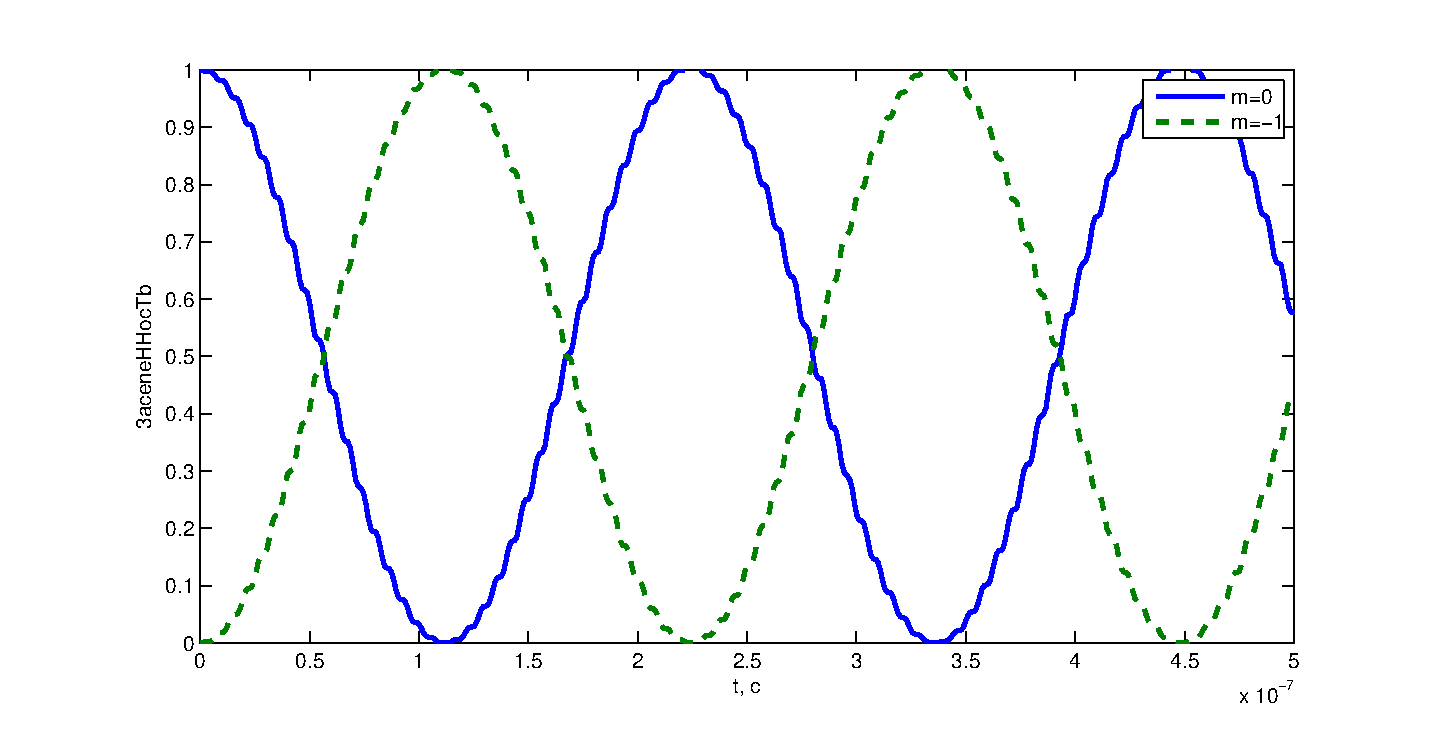
\includegraphics[width=1.1\textwidth,height=0.7\textwidth]{two_level}
  \caption{Эволюция заселенностей уровней NV-центра в двухуровневом приближении.}\label{fig:two_level}
\end{figure}


\section{Компьютерное моделирование}
Для моделирования трехуровневой системы и получения графиков была
написана программа (\ref{code}) с использованием языка программирования
Matlab. Постоянное магнитное поле заданной амплитуды направлено вдоль
оси Z и используется для расщепления по энергии уровней с проекцией
спина, равной $m$=$\pm1$. Было проведено исследование эволюции
заселенностей уровней NV-центра при различных значениях постоянного
поля (\ref{fig:spectrum}), а также различных частотах Раби.
\begin{figure}[H]\centering
  \includegraphics[width=1.1\textwidth,height=0.7\textwidth]{spectrum}
  \caption{Расщепление уровней NV-центра в магнитном поле.}\label{fig:spectrum}
\end{figure}

Прежде всего был произведен расчет в условиях, когда можно применить
приближение вращающейся волны. При амплитуде постоянного поля 350 Гс,
когда амплитуда переменного -- 30 Гс (\ref{fig:350_30}), и при
амплитуде постоянного поля 850 Гс, и амплитуде переменного 20 Гс
соответственно (\ref{fig:850_20}). Вычисления в таких условиях дадут
возможность судить о применимости аналитического решения. Из графиков
видно, что при малых частотах Раби, эволюция заселенностей уровней
NV-центра достаточно хорошо описывается двухуровневым
приближением. Паразитная заселенность уровня с $m_s$=$-1$ пренебрежимо
мала по сравнению с полезными заселенностями.
\begin{figure}[h!]\centering
  \includegraphics[width=1.1\textwidth,height=0.65\textwidth]{350_30}
  \caption{Эволюция заселенностей уровней NV-центра.}\label{fig:350_30}
\end{figure}
\begin{figure}[h!]\centering
  \includegraphics[width=1.1\textwidth,height=0.63\textwidth]{850_20}
  \caption{Эволюция заселенностей уровней NV-центра.}\label{fig:850_20}
\end{figure}

Если увеличивать частоту Раби, нарушая тем самым приближение
вращающейся волны, можно пронаблюдать поведение NV-центра, которое
нельзя получить из аналитических расчетов. Например, на графиках
(\ref{fig:350_100}) (постоянное поле 350 Гс, переменное 100 Гс) и
(\ref{fig:850_150}) (постоянное поле 850 Гс, переменное 150 Гс)
отчетливо видна паразитная заселенность уровня с проекцией спина
$m_s$=$-1$.

На графиках (\ref{fig:350_100}) - (\ref{fig:850_680}) отчетливо видны
``ступеньки'' и с увеличением частоты Раби эти ступеньки становятся
крупнее. Эти ступеньки свидетельствуют о том, что нарушается
приближение вращающейся волны.
\begin{figure}[h!]\centering
  \includegraphics[width=1.1\textwidth,height=0.67\textwidth]{350_100}
  \caption{Эволюция заселенностей уровней NV-центра.}\label{fig:350_100}
\end{figure}
\begin{figure}[h!]\centering
  \includegraphics[width=1.1\textwidth,height=0.65\textwidth]{850_150}
  \caption{Эволюция заселенностей уровней NV-центра.}\label{fig:850_150}
\end{figure}

Можно видеть, что при дальнейшем увеличение частоты Раби, паразитная
заселенность уровня с проекцией спина $m_s$=$-1$ возрастает настолько
сильно(\ref{fig:350_300}), (\ref{fig:850_680}), что говорить об успешных
однокубитных операциях не приходится. На графиках представлены расчеты
с параметрами задачи: постоянное 350 Гс, переменное -- 300 Гс и
постоянное поле 850 Гс, переменно -- 680 Гс соответственно.
\begin{figure}[h!]\centering
  \includegraphics[width=1.1\textwidth,height=0.63\textwidth]{350_300}
  \caption{Эволюция заселенностей уровней NV-центра.}\label{fig:350_300}
\end{figure}
\begin{figure}[h!]\centering
  \includegraphics[width=1.1\textwidth,height=0.6\textwidth]{850_680}
  \caption{Эволюция заселенностей уровней NV-центра.}\label{fig:850_680}
\end{figure}

Из графиков (\ref{fig:350_30}) - (\ref{fig:850_680}) видно, что скорость
операции NOT возрастает с увеличением частоты Раби. Исходя из этого
соображения частота Раби была выбрана такой, чтобы паразитная
заселенность оставалась очень малой, а скорость операции была
максимальна. Чтобы еще более ускорить операцию, было произведено
варьирование формы амплитуды микроволнового импульса.

Постоянное поле было выбрано амплитудой 850 Гс, переменное -
170 Гс. Расчеты произведены для различных форм амплитуды: прямоугольные
импульсы (\ref{fig:850_170}), импульсы в форме гауссиана
(\ref{fig:gauss}) и пилообразные импульсы (\ref{fig:saw}).
\begin{figure}[H]\centering
  \includegraphics[width=1.1\textwidth,height=0.6\textwidth]{850_170}
  \caption{Эволюция заселенностей уровней NV-центра. Прямоугольные импульсы.}\label{fig:850_170}
\end{figure}
\begin{figure}[H]\centering
  \includegraphics[width=1.1\textwidth,height=0.65\textwidth]{gauss}
  \caption{Эволюция заселенностей уровней NV-центра. Импульсы в форме гауссиана.}\label{fig:gauss}
\end{figure}
\begin{figure}[H]\centering
  \includegraphics[width=1.1\textwidth,height=0.61\textwidth]{saw}
  \caption{Эволюция заселенностей уровней NV-центра. Пилообразные импульсы.}\label{fig:saw}
\end{figure}

Как видно из графиков (\ref{fig:850_170}) - (\ref{fig:saw}), наиболее
быстрой оказывается операция NOT, произведенная под воздействием
импульсов в форме гауссиана.

На графике (\ref{fig:850_170}) в районе 6 нс видна операция NOT, но
вероятность ее осуществления только около 95\%, а в районе 14 нс
вероятность осуществления операции стремится к 100\%. В то время как
на графике (\ref{fig:gauss}) в районе 7 нс видна операция NOT с
вероятностью около 99\%.

В работе [\ref{lit:gigahertz}] были получены еще более впечатляющие
результаты. Авторы демонстрируют наносекундные операции NOT. В их
расчетах использовалось постоянное поле 850 Гс и переменное поле на
резонансной частоте. На рисунке (\ref{fig:gigahertz}) показаны
результаты, полученные при различных значениях частоты Раби.
\begin{figure}[H]\centering
  \includegraphics[height=0.9\textwidth]{gigahertz}
  \caption{``Gigahertz Dynamics of a Strongly Driven Single Quantum
  Spin''. Fuchs, Dobrovitski, Toyli, Heremans, Awschalom.}\label{fig:gigahertz}
\end{figure}

Можно видеть сильную ангармоничность заселенностей в сильных
переменных полях. При частоте Раби, равной 440 МГц, получены наиболее
быстрые осцилляции.

Моделирование системы при тех же условиях, что в работе
[\ref{lit:gigahertz}] при частоте Раби 440 МГц, показало, что
результаты, полученные в данной работе, в целом схожи с результатами
работы [\ref{lit:gigahertz}]. Однако программа (\ref{code})
демонстрирует несколько менее быстрые операции NOT. Получившиеся результаты представлены на
графике (\ref{fig:850_gigahertz}).
\begin{figure}[H]\centering
  \includegraphics[width=1.1\textwidth,height=0.65\textwidth]{850_gigahertz}
  \caption{Эволюция заселенностей уровней NV-центра. Пилообразные импульсы.}\label{fig:850_gigahertz}
\end{figure}
 % главное: произведенное исследование, результаты
\newpage
\mychapter{Обсуждение результатов}

Результаты, полученные при малых частотах Раби (\ref{fig:350_30}), (\ref{fig:850_20}), как и ожидалось,
соответствуют результатам, полученным аналитически в двухуровневом
приближении (\ref{fig:two_level}). Паразитная заселенность не
используемого уровня практически не отличима от нуля. Форма графиков
для уровней $m_s$=$0$, $m_s$=$-1$ повторяет форму для тех же уровней в
двухуровневом приближении. Таким образом можно заключить, что расчеты, произведенные
в приближении вращающейся волны, применимы для экспериментов на малых
частотах Раби.

Однако и при частотах Раби, близких к частоте резонансного перехода, но
по прежнему малых по сравнению с энергией расщепления, паразитная
заселенность остается достаточно малой (\ref{fig:350_100}), (\ref{fig:850_150}), чтобы с высокой вероятностью
производить операцию NOT. Причем при таких значениях частоты Раби
скорость этой операции значительно выше, чем при низких значениях. С
другой стороны, нельзя бесконечно ускорять операцию за счет увеличения
частоты Раби, так как заселенность неиспользуемого уровня быстро
растет с ростом частоты Раби (\ref{fig:350_300}),
(\ref{fig:850_680}). В данной работе за оптимальную частоту была
выбрана частота Раби, соответствующая амплитуде микроволнового поля
170 Гс (\ref{fig:850_170}).

Была осуществлена попытка увеличить скорость операции NOT, варьируя
форму амплитуды микроволнового поля. С помощью прямоугольных импульсов
удалось достичь длительности операции 14 нс. Пилообразный сигнал
явился более удачным: с его помощью NOT был произведен за 12
нс. Наибольшее ускорение удалось получить при использовании гауссовой
формы амплитуды. Операция NOT заняла всего 6 нс.

В работе [\ref{lit:gigahertz}] были достигнуты похожие
результаты. Кроме того, авторы подтвердили свои результаты
экспериментальными данными. NV-центр был помещен в постоянное
магнитное поле 850 Гс, а переменное поле на резонансной частоте
имело амплитуду от 29 ГГц до 440 ГГц. В первом случае наблюдались
плавные синусоидальные осцилляции Раби, как на графике
(\ref{fig:850_20}). Этот результат соответствует теории в приближении
вращающейся волны. Во случае очень сильного переменного поля (440 ГГц)
виден сильный ангармонизм в колебаниях Раби. Например, результаты
работы [\ref{lit:gigahertz}] при переменном поле 223 ГГц сильно
напоминают график (\ref{fig:850_150}).

Кроме того, авторами работы [\ref{lit:gigahertz}] было произведено
исследование при прямоугольной и гауссовой форме микроволнового
импульса. Результатом явилось сверхбыстрое (<1нс) вращение спина при
гауссовой форме импульса. В данной работе субнаносекундных спиновых
вращений обнаружить не удалось, но общие результаты соответствуют
результатам работы [\ref{lit:gigahertz}].
 % обсуждение результатов
\newpage
\chapter*{Заключение}
\addcontentsline{toc}{chapter}{Заключение}
Общепринятой практикой при расчете двухуровневых систем является
сведение более сложных систем к системам с псевдоспином $\frac{1}{2}$
в приближении вращающейся волны. В этом приближении можно пренебречь
наличием других уровней у системы, выделив два. Подобным методом в
данной работе был произведен расчет заселенностей уровней NV-центра в
аналитической части работы. В результате такого сведения был получен
рисунок (\ref{fig:two_level}). Численное моделирование трехуровневой
системы в условиях, удовлетворяющих приближению вращающейся волны,
дало очень похожие результаты, что можно наблюдать на рисунке
(\ref{fig:850_20}).

Проведенное исследование показывает, что даже при относительно больших
(порядка частоты перехода) частотах Раби остается высокая вероятность
выполнения операции NOT. Паразитная заселенность уровней пренебрежимо
мала по сравнению с ``полезными''. В качестве примера можно привести
рисунок (\ref{fig:850_150}). Это обстоятельство позволяет увеличивать
скорость операций, увеличивая частоту Раби. Однако при превышении
частотой Раби резонансной частоты перехода, паразитная заселенность
резко и быстро возрастает с ростом частоты Раби, как это видно из
рисунка (\ref{fig:850_680}). Расчет заселенностоей уровней NV-центра
при больших частотах Раби ранее производился в работе
[\ref{lit:gigahertz}]. Экспериментальные и теоретические результаты,
полученные в работе [\ref{lit:gigahertz}] показаны на рисунке
(\ref{fig:gigahertz}). Можно заметить, что графики из данной работы и
работы [\ref{lit:gigahertz}] качественно соответствуют друг другу.

Чтобы учесть неидеальность резонансного излучателя, а также
дальнейшего увеличения скорости операции NOT, были произведены расчеты
для различных огибающих резонансного излучения. В работе
[\ref{lit:gigahertz}] были рассмотрены прямоугольные импульсы и
импульсы в форме гауссиана. Последние показали очень хорошие
результаты: операцию NOT удалось произвести менее, чем за
наносекунду. В данной работе была произведена попытка отыскать еще
более удачную форму огибающей микроволнового импульса. Здесь
показаны наиболее удачные формы: прямоугольные импульсы (\ref{fig:850_170}), импульсы в
форме гауссиана (\ref{fig:gauss}) и пилообразные импульсы
(\ref{fig:saw}). Качественное соответствие результатов, полученных при
расчетах в данной работе (\ref{fig:850_gigahertz}) и экспериментальных
данных (\ref{fig:gigahertz}), полученных в работе [\ref{lit:gigahertz}],
говорит о соответствии использованной модели реальному NV-центру. В результате
исследования различных форм было выявлено, что лучшей из исследованных
является гауссовидная форма амплитуды импульса. Это еще раз подтверждает
аналогию результатов исследований проведенных в данной работе и работе
[\ref{lit:gigahertz}].


Полученные времена проведения операции NOT дают основания полагать,
что NV-центры могут стать хорошим материалом для создания кубитов в
реальных квантовых компьютерах. Такие времена операций в сравнении с
временами когерентности даже при комнатных температурах дают основания
говорить о возможности производить сотни тысяч или даже миллионы
операций над кубитом до разрушения когерентного состояния.
 % заключение
\newpage
\chapter*{Приложение}
\addcontentsline{toc}{chapter}{Приложение}
Для моделирования эволюции заселенностей NV-центра была использована
программа (\ref{code}). Расчет производился на основе
гамильтониана (\ref{eq:shamiltonian}). Форма, амплитуда и частота микроволнового
импульса подавались на вход программе, а на выходе получались данные
зависимости заселенностей уровней от времени. По этим данным были
получены представленные в работе графики.

В данном листинге представлен вариант программы, когда амплитуда
постоянного поля составляет 850 Гс. Здесь также учтены продольная и
поперечная компоненты тензора энергии расщепления в кристаллическом
поле электронных спиновых состояний.
\begin{lstlisting}[label=code, caption=NV-center model]
% @field_amplitude -- function(t) of amplitude of microwave field
% @omega -- frequency of microwave field
% @t_end -- time period during which the probabilities are calculated
%     in nanosecs
% return value -- matrix: vector t of time values, vector psi of
%     psi^2(probabilities)
function [t, psi] = test_func(field_amplitude, A, omega, t_end)
    t_end = t_end * 10^-9;
    B_z = 850;
    psi_init = [0 1 0];
    D = 2877 * 10^6;
    E = 7.7 * 10^6;
    % electron
    mu = 2.0028 * 5.788 * 10^-9;
    [t, psi] = nv_system(psi_init, D, E, mu, B_z, field_amplitude, 
                         A, omega, t_end);

    function [t, psi] = nv_system(psi_init, D, E, mu, B_z, B_0, 
                                  A, omega_field, t_end)
        h = 4.135 * 10^-15;
        t_init = 0;
        t_interval = [t_init, t_end];
        % Schrodinger equation    
        [t, psi] = ode45(@Right_part, t_interval, psi_init);
        [m,] = size(psi);
        % calculating probabilities
        for i = 1:m
            psi(i, 1) = abs(psi(i,1)^2);
            psi(i, 2) = abs(psi(i,2)^2);
            psi(i, 3) = abs(psi(i,3)^2);
        end;
    
        function dy = Right_part(t, y)
            k1 = h * D;
            k2 = h * E;
            Hamiltonian = [k1 + mu * B_z, 
                           mu * B_0(t, A) * cos(omega_field * t), 
                           2 * k2; 
                           mu * B_0(t, A) * cos(omega_field * t), 
                           0, 
                           mu * B_0(t, A) * cos(omega_field * t);
                           2 * k2, 
                           mu * B_0(t, A) * cos(omega_field * t), 
                           k1 - mu * B_z];
            dy = (Hamiltonian * y).*(-1i / h);
        end
    end
end
\end{lstlisting}
 % приложение
\newpage
\chapter*{Список литературы:}
\addcontentsline{toc}{chapter}{Список
  Литературы}
\begin{enumerate}
\item \textit{Nielsen M.A., Chuang I.L.} Quantum Computation and Quantum
Information // Cambrige: Cambrige University Press -- 2000.\label{lit:nil-chang}
\item \textit{Валиев К.А., Кокин А.А.} Квантовые компьютеры: надежды и
  реальность // 2-е изд. М. -- Ижевск: НИЦ РХД -- 2002. -- 360
  с. \label{lit:valiev-kokin}
\item \textit{Валиев К.А.} Квантовые компьютеры и квантовые вычисления //
  УФН -- 2005. -- Т. 175. -- С. 3-39.\label{lit:valiev}
\item \textit{G.D. Fuchs, V.V. Dobrovitski, D.M. Toyli, F.J. Heremans,
  D.D. Awschalom} Gigahertz Dynamics of a Strongly Driven Single
  Quantum Spin // Science 11 December -- 2009. -- V. 326. -- no. 5959
  pp. 1520-1522 DOI: 10.1126/science.1181193\label{lit:gigahertz}
\item \textit{Chuang I.L., Gershenfeld N., Kubinec M.G., Leung D.W.} Bulk
  quantum computation with nuclear magnetic resonance: theory and
  experiment //
  Proc. Roy. Soc. Lond -- 1998. -- V. A454. -- P.\label{lit:first-demonstration}
\item \textit{Robledo L., Bernien H., van Weperen I., Hanson R.} Control and
  coherence of the optical transition of single nitrogen vacancy
  venters in diamond //
  Phys. Rev. Lett -- 2010. -- V. 105. -- P. 177403.\label{lit:excitef-oscilations}
\item \textit{Collins, A.T., Thomaz, M.F., Jorge, M. I. B.}
  Luminescence decay time of the 1.945 eV centre in type Ib diamond //
  Journal of Physics -- 1983. -- C 16 (11): 2177.\label{lit:lumin-collins}
\item \textit{Hanzawa, H., Nisida, Y., Kato, T.} Measurement of decay
  time for the NV centre in Ib diamond with a picosecond laser pulse
  // Diamond and Related Materials -- 1997. -- 6 (11): 1595.\label{lit:lumin-Hanzawa}
\item \textit{Shi F., Rong X., Xu N., Wang Y., Wu J., Chong B., Peng X.,
  Kniepert J., Schoenfeld R.S., Harneit W., Feng M., Du
  J.} Room-temperature implementation of the Deutsch-Jozsa algorithm
  with a single electronic spin in diamond //
  Phys. Rev. Lett -- 2010. -- V. 105. -- P. 040504.\label{lit:nv-deutsch}
\item \textit{Цуканов А.В.} Сверхпроводящие резонаторы и зарядовые
  кубиты: спектроскопия и квантовые операции. Часть I //
  Микроэлектроника -- 2010. -- Т. 39. -- C. 404.\label{lit:tsukanov-super-cond-one}
\item \textit{Цуканов А.В.} Сверхпроводящие резонаторы и зарядовые кубиты:
  спектроскопия и квантовые операции. Часть II //
  Микроэлектроника -- 2011. -- Т. 40. -- C. 11.\label{lit:tsukanov-super-cond-two}
\item \textit{Yamamoto Y., Ladd T.D., Press D.,  Clark S., Sanaka K., Santori
  C., Fattal D., Fu K.M., Höfling S., Reitzenstein S., Forchel
  A.} Optically controlled semiconductor spin qubits for quantum
  information processing //
  Phys. Scripta -- 2009. -- V. T139. -- P. 014010.\label{lit:dots}
\item \textit{Kane B.E.} A silicon-based nuclear spin quantum computer //
  Nature -- 1998. -- V. 393. -- P. 133.\label{lit:implant}
\item \textit{Monz, Thomas} 14-Qubit Entanglement: Creation
  and Coherence // Physical Review Letters (American Physical
  Society) -- 2011. -- March 31\label{lit:ion-trap}
\end{enumerate}

 % список литературы
\end{document}
